\documentclass{article}

\usepackage{hyperref}
\newcommand*{\et}[0]{\textit{et~al. }}
\newcommand*{\fig}[1]{Fig.~\ref{fig:#1}}
\newcommand*{\Fig}[1]{Figure~\ref{fig:#1}}


%%% This file is the preamble for the Pomona Linguistics LaTeX Paper Template, which is also used for the Quick Reference Guide. If you are brand new to writing with LaTeX, we suggest NOT messing with it, and just writing your paper using the Paper Template. If you are getting more comfortable in LaTeX and want to add packages and commands, this is where you do it (when using this template).

%For stacking text, used here in autosegmental diagrams
\usepackage{stackengine}

%To combine rows in tables
\usepackage{multirow}

%geometry helps manage margins, among other things.
\usepackage[margin=1in]{geometry}

%Gives some extra formatting options, e.g. underlining/strikeout
\usepackage{ulem}

%For putting links into papers, also helps make cross-references in the paper smart references
\usepackage[colorlinks = true,
            linkcolor = blue,
            urlcolor  = blue,
            citecolor = blue,
            anchorcolor = blue]{hyperref} %smarter cross-references, these options turn links blue

%Use package/command below to create a double-spaced document, if you want one. Uncomment BOTH the package and the command (\doublespacing) to create a doublespaced document, or leave them as is to have a single-spaced document.
%\usepackage{setspace}
%\doublespacing 

%paragraph formatting
\usepackage[parfill]{parskip}
\setlength{\parskip}{5pt} %plus 1 minus 1}
\setlength{\parindent}{30pt}
\usepackage{titlesec}

%use for special OT tableaux symbols like bomb and sad face. must be loaded early on because it doesn't play well with some other packages
\usepackage{fourier-orns}

%Basic math symbols 
\usepackage{pifont}
\usepackage{amssymb}

%%%Gives shortcuts for glossing. The use of this package is NOT explained in the Quick Reference Guide, but the documentation is on CTAN for those that are interested. MJKD finds it handy for glossing. (https://ctan.org/pkg/leipzig?lang=en)
\usepackage{leipzig}

%Tables
\usepackage{caption} %For table captions
\usepackage{booktabs} %helps format tables

%For citations and bibliography - as of 9.1.2019 we don't explain citations in this Quick Reference Guide, but Pedro Martin's tutorial does (see links in the Guide).
\usepackage{natbib}

%For OT-style tableaux
\usepackage{ot-tableau}

%Fonts
\usepackage[no-math]{fontspec} %This allows you to enter (via an IPA kayboard) IPA fonts and other symbols directly into LaTeX. Requires a particular setyp, see below.
\usepackage{libertine} %A font that actually contains many IPA symbols. This is the font you see in the preview to the right.

%to use these fonts, be sure that your typesetting engine is set to "XeLaTeX." In Overleaf, go to the Menu link on the top left (by the Overleaf icon), and under Settings be sure that the Compiler is set to "XeLaTeX." If you accessed this document via the Overleaf Pomona Linguistics template, all of this was already done for you.

%The Pomona Linguistics Paper Template in Overleaf is already set up for this, but you may run into this problem if you start building your own documents.

%highlights text with \hl{text}
\usepackage{color, soul}

%Drawing Syntax Trees
\usepackage[linguistics]{forest}

%This specifies some formatting for the forest trees to make them nicer to look at
\forestset{
  nice nodes/.style={
    for tree={
      inner sep=0pt,
      fit=band,
    },
  },
  default preamble=nice nodes,
}

%% For numbered and glossed examples %%
\usepackage{gb4e}



%Changes the \maketitle command to be smaller and take up less space on a page. 
\makeatletter         
\def\@maketitle{   % custom maketitle 
\noindent {\Large \bfseries \color{black} \@title}  \\ \hrule \noindent \@author \\ %\@date
}

%The code below will draw a circle around a piece of text. This is very useful for drawing attention to a word in a data example. use the command \circled{text} where the argument (`text' here) is what you want to be circled. This is illustrated in the Quick Reference Guide and the Paper Template.

\usepackage{tikz}

\newcommand{\circled}[1]{\begin{tikzpicture}[baseline=(word.base)]
\node[draw, rounded corners, text height=8pt, text depth=2pt, inner sep=2pt, outer sep=0pt, use as bounding box] (word) {#1};
\end{tikzpicture}
}


%%%%%%%%%%%%%%%%%%%%%%%%%%%%%%%%%%%%%%%%%%%%%%%%%%%%%%%%%%%%
%%%%%%%%%%%%%%%%%%%%%%%%%%%%%%%%%%%%%%%%%%%%%%%%%%%%%%%%%%%%

% Useful Ling Shortcuts

\RequirePackage{leipzig}
%\RequirePackage{mathtools} % for \mathrlap

% % % Shortcuts  (borrowed from JZ, I'm still unsure exactly what xspace requires)
\RequirePackage{xspace}
\xspaceaddexceptions{]\}}

%This makes the \emptyset command be a nicer one
\let\oldemptyset\emptyset
\let\emptyset\varnothing
\newcommand{\nothing}{$\emptyset$}

%Not all of these are explained in the Quick Reference Guide, but they are here bc they are relevant to some of our students.
\newcommand{\1}{\rlap{$'$}\xspace}
\newcommand{\0}{\rlap{\textsuperscript{$ˆ{\circ}$}}\xspace}
\newcommand{\Lb}[1]{$\text{[}_{\text{#1}}$ } %A more convenient left bracket
\newcommand{\Rb}[1]{$\text{]}_{\text{#1}}$ } %A more convenient left bracket
\newcommand{\gap}{\underline{\hspace{1.2em}}}
\newcommand{\vP}{\emph{v}P}
\newcommand{\lilv}{\emph{v}}
\newcommand{\Abar}{A$'$-} %A more convenient A-bar notation
\newcommand{\ph}{$\varphi$\xspace} %A more convenient phi
\newcommand{\pro}{\emph{pro}\xspace}
\newcommand{\subs}[1]{\textsubscript{#1}} %A more convenient subscript
%\newcommand{\hd}{$^{\circ}$\xspace} %Symbol for printing head / degree symbol
\newcommand{\spells}{$\Longleftrightarrow$} %spellout arrow for morph spellout rules
\newcommand{\tr}[1]{\textit{t}\textsubscript{\textit{#1}}} %easy traces with subscript
\newcommand{\supers}[1]{\textsuperscript{#1}}

% Abbreviations for glossing, based on Leipzig
\newleipzig{hab}{hab}{habitual}
\newleipzig{rem}{rem}{remote}
\newleipzig{sm}{sm}{subject marker}
\newleipzig{t}{t}{tense}
\newleipzig{aa}{aa}{anti-agreement}
\newleipzig{pron}{pron}{pronoun}
\newleipzig{rec}{rec}{recent}
\newleipzig{om}{om}{object marker}
%\newleipzig{ipfv}{ipfv}{imperfective}
\newleipzig{asp}{asp}{aspect}
\newleipzig{lk}{lk}{linker}
\newleipzig{pcl}{pcl}{particle}
\newleipzig{stat}{stat}{stative}
\newleipzig{ints}{ints}{intensive}
\newleipzig{ascl}{ascl}{assertive subject clitic}
\newleipzig{nascl}{nascl}{non-assertive subject clitic}
\newleipzig{ta}{ta}{tense and/or aspect}
\newleipzig{assoc}{assoc}{associative marker}
\newleipzig{hon}{hon}{honorific}
%\newleipzig{whprt}{wh}{\wh particle}
\newleipzig{sa}{sa}{subject agreement}
\newleipzig{conj}{conj}{conjunction}
%\newleipzig{loc}{loc}{locative}
\newleipzig{expl}{expl}{expletive}
\newleipzig{rcm}{rcm}{reciprocal marker}
\newleipzig{pers}{pers}{persistive}
%\newleipzig{}{}{} %this is just to copy for when I want to add more

%%%%%%%%%%%%%%%%%%%%%%%%%%%%%%%%%%%%%%%%%%%%%%%%%%%%%%%%%%%%
%%%%%%%%%%%%%%%%%%%%%%%%%%%%%%%%%%%%%%%%%%%%%%%%%%%%%%%%%%%%

%A couple of packages that seemed to prefer being called toward the end of the preamble

%This package provides macros for typesetting SPE-style phonological rules.
\usepackage{phonrule}

%For using Greek letters outside of math mode.
\usepackage{textgreek}


%Random, lets us use the XeLaTeX logo. Not important to the template at all.
\usepackage{metalogo}


%%%%%%%%%%%%
%% This is the end of the PREAMBLE
%%%%%%%%%%%


\title{Million Songs Decade Prediction}
\author{Shahriar Hooshmand}
%\date{\today} 

\begin{document}

\maketitle

\section*{Project Statement}

With the relatively recent boom in music streaming and digital music sales, interest in music data mining has steadily increased. Audio, in the form of waveform data files, can be segmented into numerous features such as pitch, tempo and loudness, as well as contrived metrics like ``danceability" and ``energy". Machine learning analysis of these features is of great interest to the industry for determining things like target market demographics and suggested songs lists. 

\noindent In this project, various classifiers are applied to the determine the decade of songs in which they were released. The dataset for the problem is \href{http://millionsongdataset.com}{Columbia's Labrosa laboratory's} ``1 million song \href{https://archive.ics.uci.edu/ml/datasets/yearpredictionmsd}{dataset}". Of the 1 million songs, $515,345$ had known years associated to them, although only a subset were used for training purposes due to time constraints. Splitting this dataset, we had 10 classes between 1920's-2010's, with the 2000's being the most common choice. We used $3$ classifiers detailed below: Multiclass support vector machines (SVM), Adaboost and multi-layer neural network (NN). 

\section*{Baseline}

If a classifier were to guess 2000's everytime, it would achieve $58.02\%$ ($299,003/515,345$) accuracy. This is considered as our baseline here. SVM and NN are both parametric methods that can embed non-linearity. Since we are dealing with large dataset, NN accuracy can become comparable to SVM and this would be a good exercise to evaluate and compare the convergence speed vs accuracy between these two methods. To avoid the overfitting and enhance the predictivity power of the model, Adaboost is also employed. This method is easier to use with less need for tweaking parameters, unlike NN and SVM and would be a good baseline for the comparison. 

\section*{SVM}
\underline{Dataset}: The dataset was split into training, validation and test sets. Training and validation sets together contained the first $463,715$ samples while test set contained the last $51,630$ samples. This split was recommended on UCI's website to avoid producer effect which makes sure that no song from a given artist ends up being used for both training and testing. 

\noindent SVC and NuSVC implement 1 vs 1 approach for multi-class classification i.e. if $n$ is the number of classes, then $\frac{n(n-1)}{2}$ models are constructed where as LinearSVC implement 1 vs rest multi-class strategy, thus training only $n$ models. 1 vs rest strategy is usually preferred in practice, and yields similar results for significantly less runtime. Based on this information from Scikit-learn's manual \cite{buitinck2013}, LinearSVC was used for classification. 

\noindent  \underline{Parameter tuning}: $500$ randomly selected samples from the first $90 \, \%$ samples were used to construct the validation set with the remaining samples in training set. Parameter tuning was done using GridSearchCV for $3-$fold cross-validation. The maximum number of allowed iterations was 1 million. Parameter tuning was done on cost values between $2^{-4}$ and $2^8$, and primal hinge loss versus dual hinge loss. The optimal accuracy was with $2^{-1}$ and dual hinge loss at $0.45$ (details in Appendix table 1). 

\noindent  \underline{Results}: The best parameters obtained after parameter tuning on validation set were used to train and test LinearSVC. The detailed classification results on test set can be found in Appendix Table 2. Precision $tp/(tp+fp)$, recall $tp/(tp+fn)$, f1-score (harmonic mean of precision and recall) and support (number of occurrences of corresponding class), where $tp, fp$, and $fn$ are true positive, false positive and false negative, respectively are included for each of the 10 classes i.e. 10 decades from 1920s to 2010s. The reported averages include micro avg (averaging the total tp, tn and fp), macro avg (averaging the unweighted mean per class) and weighted avg (averaging the support-weighted mean per class). Accuracy on entire test set was $56 \%$ with a total running time (including data loading and parameter tuning) of $\sim 8$ minutes. 

\section*{Adaboost}

Using scikit's implementation of Adaboost with decision stumps as the model classifier, the same analysis detailed above for SVM is employed. Testing on $63,345$ data samples, there was almost no difference in accuracy for $10, 50, 100, 300, 500$, and $1000$ weak classifiers on the same data split. The maximum accuracy was $59 \%$, just slightly above the baseline. 


\section*{Neural network analysis}

Multi-layer perceptron (MLP) feature within scikit-learn package has been used to build the model, train and test over the dataset. Given a set of features $X_i$ and target tags $y$, MLP can learn non-linear function approximator for classification and regression. While MLP classifiers have the capability to learn non-linear models in real time, due to a non-convex loss function where there exists more than one local minimum, it is of crucial importance to perform parameter tuning in these type classifiers. Using the scripts we wrote, extensive parameter tuning analyses performed on the number of hidden layers, neurons within each layer, learning rate and regularization term. Our measurement criteria of accuracy and performance efficiency are on number of epochs, training and validation errors. 

\noindent We use stochastic based optimizer developed by Kingma \et \cite{kingma2017} with the optimization tolerance of $1e-4$. We find a better accuracy using logistic sigmoid while the results are not super sensitive to different minimization algorithms. \Fig{fig1} shows the contour plot of parameter tuning analysis on the number of hidden layers and neurons. This analysis includes $40 \times 40$ calculations and as this type analysis is computationally demanding, we did the parameter tuning on a toy set of $500$ data. Our observation shows that the use of large number of hidden layers decrease the model accuracy and this is expected due to the vanishing gradient phenomenon. We find that $2$ hidden layers with $39$ neurons within each layer gives an accuracy of $72-78 \%$ which is a fair range and use this settings for our model implementation. 



\begin{figure}[h!] % Figure at bottom of the page ([b] argument, could be "t" for top or "h" for here)
	\centering
	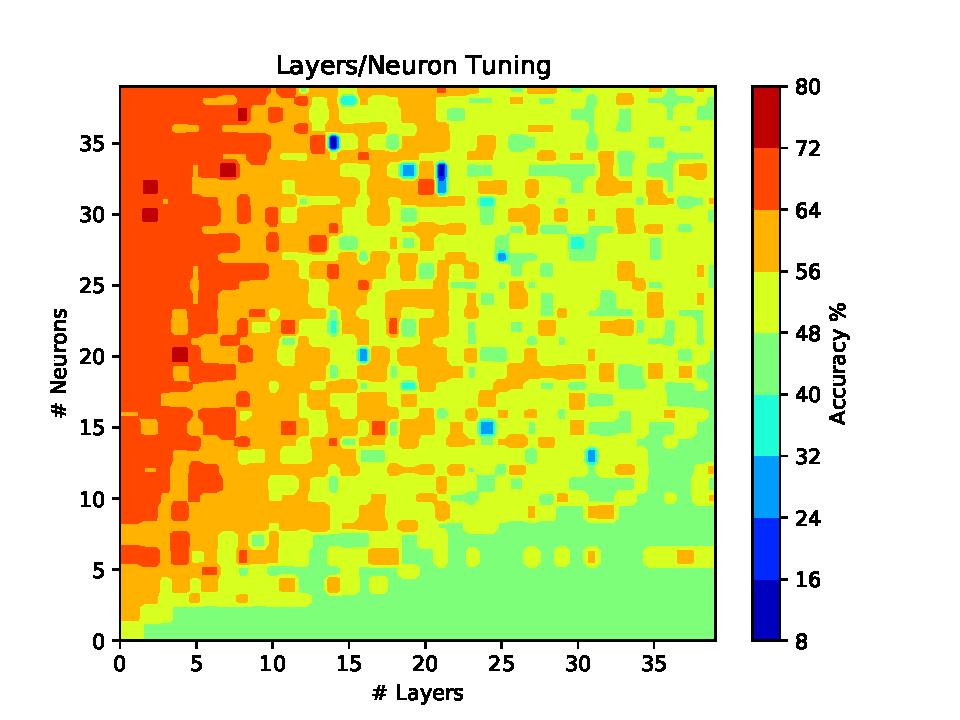
\includegraphics[scale = .50]{figs/contour.pdf}
	\caption{\footnotesize Contour plot of parameter tuning on the number of hidden layers and neurons within each layer.}
	\label{fig:fig1}
\end{figure}

\noindent  Next, we did some analysis on learning grate $\eta$ and L$2$ regularization $\alpha$ parameters. Choosing the optimum learning rate is important in the minimization algorithm to avoid trapping in local metastable minima. $\alpha$ terms in gradient descent is added to weight update within back-propagation algorithm to ease the oscillation of weights due to the large learning rates. In fact, in downhill situation learning is accelerated by the factor of $1/(1-\alpha)$. \Fig{fig2} shows the results after examining different learning rates in the range of $0.1$ to $0.5$ and momentum term of $0$ to $0.9$. Higher $\eta$ and $\alpha$ have shown the speed up the convergence, however the training error decreases in very large $\eta$ values. We find that $\eta=0.1$ and $\alpha=0.5$ are the optimum parameters for our model with the $70-75 \%$ accuracy on the training data. 

\begin{figure}[h!]% Figure at bottom of the page ([b] argument, could be "t" for top or "h" for here)
	\centering
	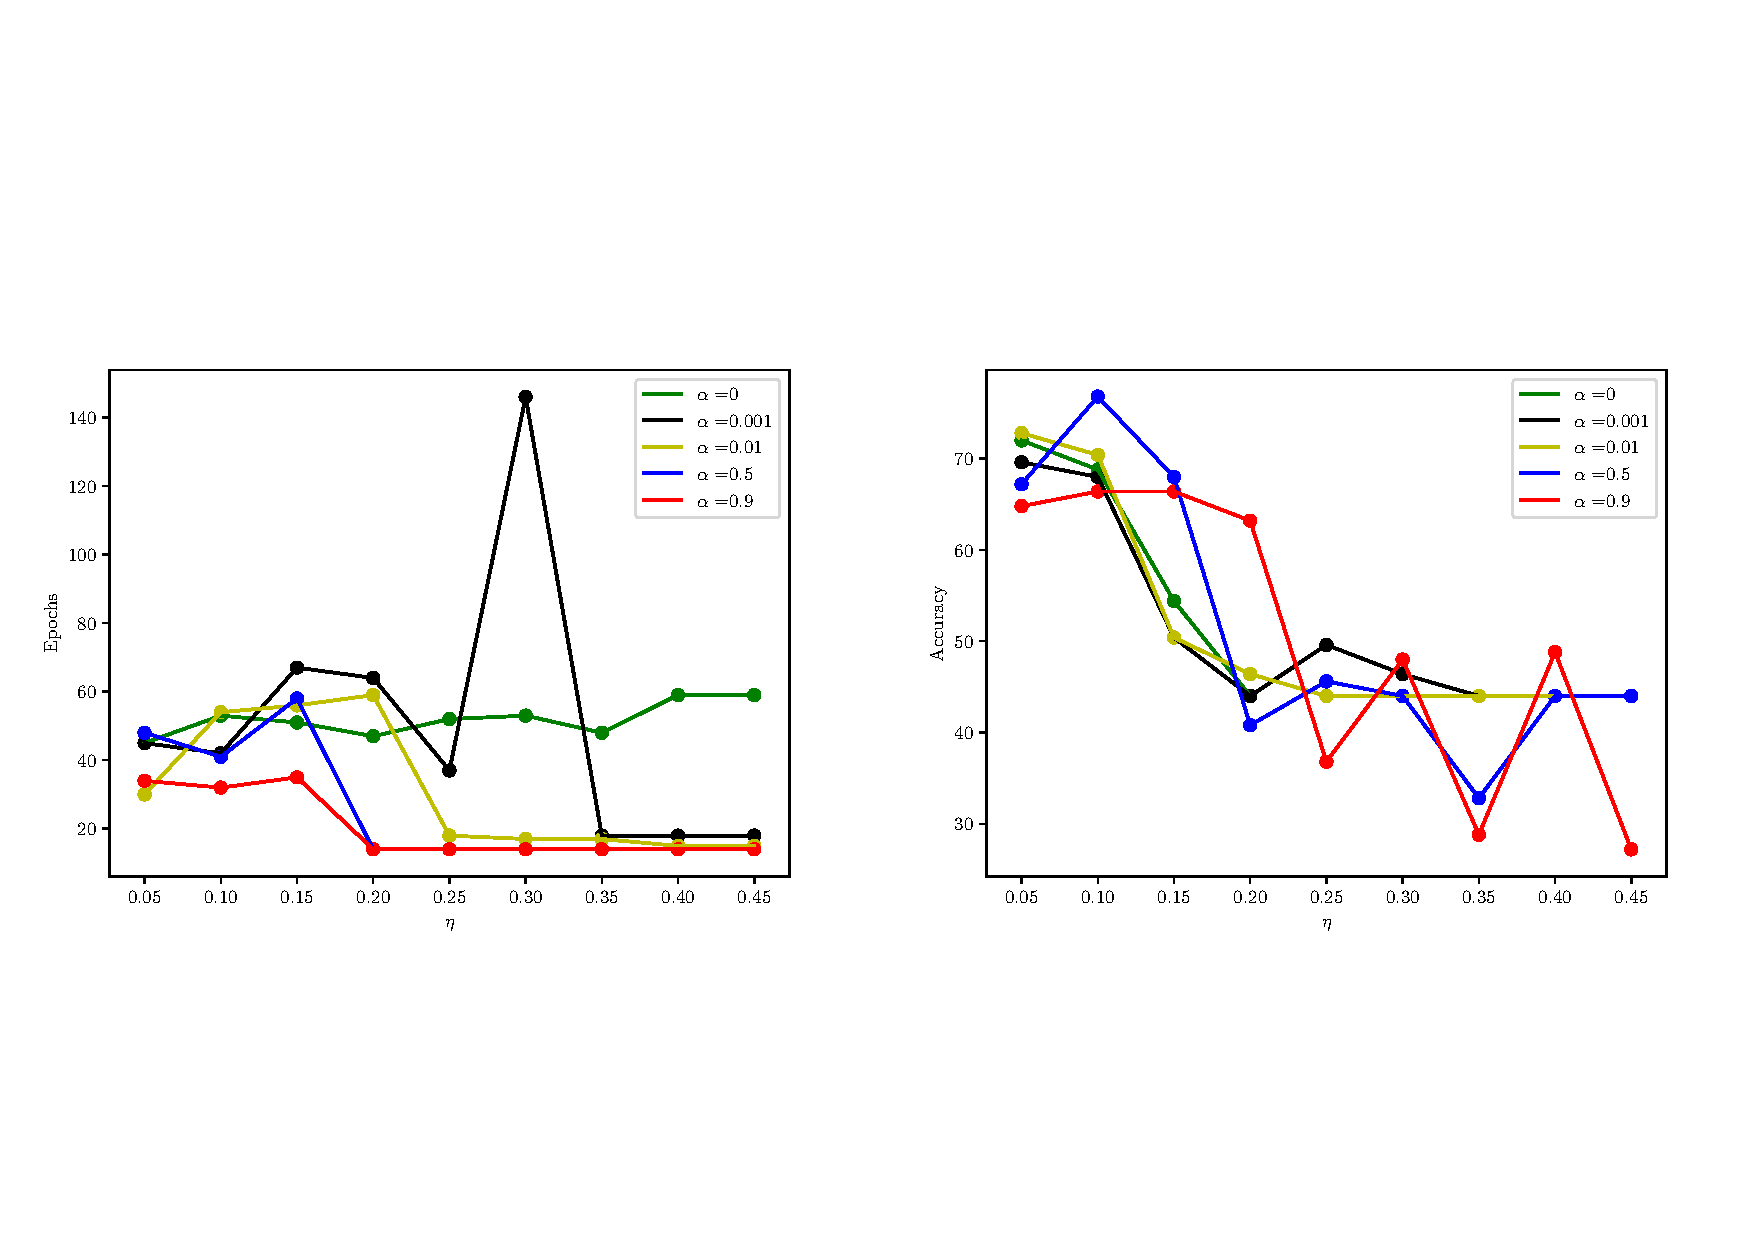
\includegraphics[width=\textwidth]{figs/params.pdf}
	\caption{\footnotesize Parameter tuning on the learning rate and regularization parameter. Number of epochs till the convergence and the cross validation accuracy for each parameter are shown in left and right panels, respectively. }
	\label{fig:fig2}
\end{figure}

\noindent  Now that we tuned the parameters of our MLP model, we implement the cross validation algorithm to train on $75\%$ of dataset and test on the remaining $25\%$ of unseen data. The final cross-validated accuracy of  decade prediction of songs is $74\%$. This accuracy is unique on such a large dataset with more than 90 features associated with each song. More in-depth analysis can be also performed to better optimize the mode given more advanced and powerful supercomputing resources. 

\section*{Overall conclusion}

We achieved a set of accuracy of about $74\%$ for the optimized neural network, which is significantly larger than the baseline. For such a large dataset, this is a fairly significant improvement. 

%\section*{References}
\bibliographystyle{plain}
% \bibliographystyle{nature}

\bibliography{bib.bib}

\pagebreak
\newpage
\clearpage

\section*{Appendix}

\begin{table}[ht]
\caption{Detailed SVM classification results  }

\label{tab1}
\centering
\begin{tabular}{lllll}
\hline
             & Precision & Recall & f1-score & Support \\ \hline
1920         & 0.02      & 0.65   & 0.05     & 20      \\
1930         & 0.01      & 0.54   & 0.02     & 13      \\
1940         & 0.02      & 0.49   & 0.05     & 61      \\
1950         & 0.05      & 0.45   & 0.09     & 275     \\
1960         & 0.16      & 0.35   & 0.22     & 1166    \\
1970         & 0.26      & 0.35   & 0.30     & 2396    \\
1980         & 0.36      & 0.44   & 0.40     & 4201    \\
1990         & 0.51      & 0.11   & 0.18     & 12580   \\
2000         & 0.73      & 0.81   & 0.77     & 29885   \\
2010         & 0.00      & 0.00   & 0.00     & 1033    \\ \hline
             &           &        &          &         \\ \hline
micro avg    & 0.56      & 0.56   & 0.56     & 51630   \\
macro avg    & 0.21      & 0.42   & 0.21     & 51630   \\
weighted avg & 0.59      & 0.56   & 0.54     & 51630   \\ \hline
\end{tabular}
\end{table}




\begin{table}[ht]
\caption{Detailed SVM parameter optimization }

\label{tab2}
\centering
\begin{tabular}{lllllllllllll}
\hline
                                                                    & -4  & -3  & -2  & -1  & 0   & 1   & 2   & 3   & 4   & 5   & 6   & 7   \\ \hline
\begin{tabular}[c]{@{}l@{}}loss=sq\_hinge\\ dual=False\end{tabular} & .42 & .42 & .44 & .45 & .44 & .44 & .44 & .44 & .44 & .44 & .44 & .44 \\
\begin{tabular}[c]{@{}l@{}}loss=hinge\\ dual=True\end{tabular}      & .38 & .37 & .41 & .41 & .42 & .42 & .42 & .42 & .42 & .43 & .43 & .43 \\ \hline
\end{tabular}
\end{table}

\end{document}
